\documentclass[12pt]{article}

\usepackage{geometry}
\usepackage{fancyhdr}
\usepackage{extramarks}
\usepackage{amsmath}
\usepackage{amsthm}
\usepackage{amsfonts}
\usepackage{amssymb}
\usepackage{tikz}
\usepackage[plain]{algorithm}
\usepackage{algpseudocode}
\usepackage{fancyhdr}
\usepackage{array}
\usepackage{wrapfig}
\usepackage{adjustbox}
\usepackage{enumitem}
\usepackage{tasks}


\newlength{\strutheight}
\settoheight{\strutheight}{\strut}
\newtheorem{theorem}{Theorem}
\renewcommand\qedsymbol{$\blacksquare$}
\newcommand\setitemnumber[1]{\setcounter{enumi}{\numexpr#1-- -1\relax}}

\geometry{letterpaper,portrait,margin=1in}


\title{\large Historical Roots of Mathematics Homework 2}
\author{\large Zachary Meyner}
\date{}

\begin{document}
\maketitle
\begin{enumerate}[label=\textbf{\arabic*}.]
    \item In problem 30 of the Rhind Papyrus the area of a circle is eqated to the square of $\displaystyle\frac{8}{9}$ of 
    the diameter. Prove that this leads to the approximation $\pi\approx\displaystyle\frac{256}{81}$
    \begin{proof}
        Consider a circle with radius $r$ and diameter $d=2r$. Consider the approximation of the area 
        \[A \approx {\bigg(=\frac{8}{9}\bigg)}^{2}d\]
        Then we know
        \begin{align*}
            A = \pi r^{2} &\approx {\bigg(\frac{8}{9}\cdot d\bigg)}^{2} \\
            \pi r^{2} &\approx {\bigg(\frac{8}{9}\cdot 2r\bigg)}^{2} && (d = 2r) \\
             \pi r^{2} &\approx {\bigg(\frac{16}{9}r\bigg)}^{2}  \\
            \pi r^{2} &\approx \frac{256}{81}r^{2} \\
            \pi &\approx \frac{256}{81}
        \end{align*}
    \end{proof}
    \item Calcualte using the Egyptian method:
    \begin{enumerate}
        \item 
        \begin{tasks}[label=] (2)
            \task$12 \div 23$
        \begin{align*}
            &1 & 23 \\
            \checkmark&\overline{2} & 11 + \overline{2} \\
            \checkmark&\overline{46} & \overline{2}
        \end{align*}
        \task$1 \div 2 $
        \begin{align*}
            \checkmark&\overline{2} & 1
        \end{align*}
    \end{tasks}
    $12 \div 23 = \overline{2} + \overline{46}$
    \pagebreak
    \item
    \begin{tasks}[label=] (2)
        \task$11 \div 13$
        \begin{align*}
            &1 & 13 \\
            \checkmark&\overline{3} & 4 + \overline{3} \\
            \checkmark&\overline{2} & 6 + \overline{2} \\
            \checkmark&\overline{78} & \overline{6}
        \end{align*}
        \task{Complete} $10 + \overline{3} + \overline{2}$ to $11$ \\
        Complete $\overline{3} + \overline{2}$ to $1$ \\
        Sum: $5$ Remainder: $1$\\
        $1 \div 6$
        \begin{align*}
            \checkmark&\overline{6} & 1
        \end{align*}
    \end{tasks}
    $1 \div 6 = \overline{78} + \overline{3} + \overline{2}$
    \item 
    \begin{tasks}[label] (2)
        \task$15 \div 19$
        \begin{align*}
            &1 & 19 \\
            \checkmark&\overline{2} & 9 + \overline{2} \\
            \checkmark&\overline{4} & 4 + \overline{2} + \overline{4} \\
            \checkmark&\overline{38} & \overline{2} \\
            \checkmark&\overline{76} & \overline{4} 
        \end{align*}
        \task{Complete} $14 + \overline{4}$ to 15 \\
        Complete $\overline{4}$ to 1 \\
        Sum:1 Remainder 3 \\
        $3 \div 4$
        \begin{align*}
            &1 & 4 \\
            \checkmark&\overline{2} & 2 \\
            \checkmark&\overline{4} & 1
        \end{align*}
    \end{tasks}
    $15 \div 19 = \overline{76} + \overline{38} + \overline{4} + \overline{2}$
    \item 
    \begin{tasks}[label=] (2)
        \task$33 \div 7$
        \begin{align*}
            &1 & 7 \\
            &2 & 14 \\
            \checkmark&4 & 28 \\
            \checkmark&\overline{\overline{3}} & 4 + \overline{\overline{3}} \\
            \checkmark&\overline{21} & \overline{3}
        \end{align*}
        \task{Complete} $32 + \overline{\overline{3}}$ to 33 \\
        Complete $\overline{\overline{3}}$ to 1 \\
        Sum: 2 Remainder 1 \\
        $1 \div 3$
        \begin{align*}
            \checkmark&\overline{3} & 1
        \end{align*}
    \end{tasks}
    $33 \div 7 = 4 + \overline{21} + \overline{\overline{3}}$
    \item 
    \begin{tasks}[label=] (2)
        \task$11 \div 65$
        \begin{align*}
            &1 & 65 \\
            &\overline{3} & 21 + \overline{\overline{3}} \\
            \checkmark&\overline{6} & 10 + \overline{2} + \overline{3} \\
            \checkmark&\overline{390} & \overline{6}
        \end{align*}
        \task{Complete} $10 + \overline2 + \overline3$ to 11 \\
        Complete $\overline2 + \overline3$ to 1 \\
        Sum: 5 Remainder: 1
        $1 \div 6$
        \begin{align*}
            \checkmark&\overline6 & 1
        \end{align*}
    \end{tasks}
    $11 \div 65 = \overline{390} + \overline6$
    \item 
    \begin{tasks}[label=] (2)
        \task$9 \div 23$
        \begin{align*}
            &1 & 23 \\
            &\overline{2} & 11 + \overline2 \\
            \checkmark&\overline3 & 7 + \overline{\overline3} \\
            \checkmark&\overline{23} & 1 \\
            \checkmark&\overline{69} & \overline{3}
        \end{align*}
        \task{Complete} $8 + \overline{\overline{3}}$ to 9.\\
        Complete $\overline{\overline3}$ to 1 \\
        Sum: 2 Remainder: 1
        $1 \div 3$
        \begin{align*}
            \checkmark&\overline{3} & 1
        \end{align*}
    \end{tasks}
    $9 \div 23 = \overline{69} + \overline{23} + \overline3$
\end{enumerate}
    \item Solve the following problems from the Cairo Papyrus (300 BC):
    \begin{enumerate}
        \item A ladder of 10 cubuts has its foot 6 cubits from a wall. To what height does the 
        ladder reach? \\
        \(\begin{aligned}
            a^2 + 6^2 = 10^2 \\
            a^2 + 36 = 100 \\
            a^2 = 64 \\
            a = 8
        \end{aligned} \) \qquad \qquad \qquad \qquad
        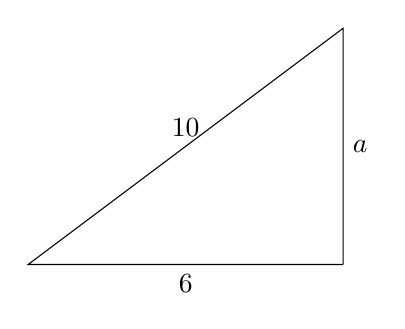
\begin{tikzpicture}[baseline=4ex]
            \draw (0,0) -- (-4,0) node[midway, below] {$6$} 
            -- (0, 3) node[midway, above] {$10$}
            -- (0,0) node[midway, right] {$a$};
        \end{tikzpicture}
        \item A rectangle with an aera of 60 square cubits has a diagonal of 13 cubits. Find 
        the sides of the rectangle. \\
        \(\begin{aligned}
            a \cdot b = 60 \\
            a^2 + b^2 = 169\\
            5 \cdot 12 = 60\\ 
            5^2 + 12 ^2 = 25 + 144 = 169
        \end{aligned}\) \qquad \qquad \qquad 
        \begin{tikzpicture}
            \draw (0,0) -- (5,0) node[midway, below] {$a$} 
            -- (5,3) node[midway, right] {$b$}
            -- (0,3) 
            -- (0,0);
            \draw (0,0) -- (5,3) node[midway, above] {$13$};
            \draw (3.2,1) node {$60$};
        \end{tikzpicture}
        \pagebreak
        \item A rectangle with an aera of 60 square cubits has a diagonal of 15 cubits. Find 
        the sides of the rectangle. \\
        \(\begin{aligned}
            a \cdot b = 60 \\
            a^2 + b^2 = 225\\
            a^2 + 2ab + b^2 = 225 + 2ab\\
            a^2-2ab +b ^2 = 225-2ab \\
            \begin{cases}
                a+b = \sqrt{345} \\
                a-b = \sqrt{105}
            \end{cases} \\
            2a = \sqrt{345} - \sqrt{105} \\
            \begin{cases}
            a = \frac{\sqrt{345}-\sqrt{105}}{2}\\
            b = \frac{60}{\frac{\sqrt{345}-\sqrt{105}}{2}}
            \end{cases}
        \end{aligned}\) \qquad \qquad \qquad 
        \begin{tikzpicture}
            \draw (0,0) -- (5,0) node[midway, below] {$a$} 
            -- (5,3) node[midway, right] {$b$}
            -- (0,3) 
            -- (0,0);
            \draw (0,0) -- (5,3) node[midway, above] {$15$};
            \draw (3.2,1) node {$60$};
        \end{tikzpicture}
    \end{enumerate}
    \item Use the method of false position to solve the following problems from the \\Rhind 
    Papyrus. Express your answers in unit fractions.
    \begin{enumerate}
        \item A quantity and its fourth, added together, give 15. What is the quantity?
        \[x+\frac{x}{4} = 15\]
        Guess 8:
        \[8 + \frac{8}{4} = 10\]
        $15 \div 10$
        \begin{align*}
            \checkmark&1 & 10 \\
            \checkmark&\overline{2} & 5
        \end{align*}
        $15 \div 10 = 1 + \overline{2}$
        \[8(1+\overline{2}) = 12 \]\[x = 12 \]
        \item A quantity and its fifth, added together, give 21. What is the quantity?
        \[x + \frac{x}{5} = 21\]
        Guess 15:
        \[15 + \frac{15}{5} = 18\]
        $21 \div 18$
        \begin{gather*}
            21-18=3 \\ 
            1 + \frac{3}{18} = 1+\frac{1}{6}
        \end{gather*}
        \[15(1+\frac{1}{6}) = 15 + \frac{15}{6} = 17 + \frac{3}{6} = 17 + \frac{1}{2}\]
        \[x = 17 + \frac{1}{2}\]
    \end{enumerate}
\end{enumerate}

\end{document}